
\appendix
\renewcommand{\thechapter}{\Alph{chapter}}
\renewcommand{\chaptername}{Appendice}

\titleformat{\chapter}[display]
  {\normalfont\huge\bfseries\centering} % titolo centrato
  {Appendice \thechapter} % qui \thechapter darà A, B, ...
  {20pt}
  {{\Huge\justifying}}
  []
%\raggedright % Forza allineamento a sinistra

\chapter{Confronto visivo tra modelli} \label{chap:appendice_risultati}
In questa appendice sono riportati i risultati qualitativi ottenuti
sui diversi dataset con i tre modelli di denoising addestrati:
\textbf{Ridnet}, \textbf{DnCNN} e \textbf{Autoencoder}, e \textbf{BM3D}.
Per ogni dataset e livello di rumore si confrontano le uscite dei modelli.

% -------------------------------------------------------
% Definizione dei modelli
\def\models{{ridnet},{dncnn},{autoencoder},{bm3d}}

% -------------------------------------------------------
% Dataset con un solo livello di rumore
\foreach \dset in {renoir, sidd}{%
  \begin{sidewaysfigure}[h!]
    \centering
    \foreach \m [count=\i] in \models {%
      \begin{subfigure}{0.48\textwidth}
        \centering
        \includegraphics[width=\linewidth]{img/psnr/\m/\m_\dset.png}
        \caption{\m}
      \end{subfigure}\hspace{2em} % spazio orizzontale tra due subfigure
      \ifodd\i\else \par\vspace{2ex}\fi % va a capo con spaziatura verticale maggiore
    }
    \caption{Dataset \dset}
  \end{sidewaysfigure}
}

% -------------------------------------------------------
% Dataset con tre livelli di rumore
\foreach \dset in {bsd,fivek,div2k}{%
  \foreach \n in {15,25,50}{%
    \begin{sidewaysfigure}[h!]
      \centering
      \foreach \m [count=\i] in \models {%
        \begin{subfigure}{0.48\textwidth}
          \centering
          \includegraphics[width=\linewidth]{img/psnr/\m/\m_\dset_\n.png}
          \caption{\m}
        \end{subfigure}\hspace{2em} % spazio orizzontale tra subfigure
        \ifodd\i\else \par\vspace{2ex}\fi % spazio verticale maggiore tra le righe
      }
      \caption{Dataset \dset – Livello di rumore $\sigma=\n$.}
    \end{sidewaysfigure}
  }
}

\chapter{Risultati Fine Tuning}
\label{chap:finetuning_results}
Qui di seguito sono riportati i risultati visivi pre e post fine tuning sul dataset Kvasir, per i tre modelli addestrati: \textbf{Ridnet}, \textbf{DnCNN} e \textbf{Autoencoder}, e \textbf{BM3D}.

% -------------------------------------------------------
% Dataset con tre livelli di rumore
\def\modelss{ridnet, dncnn, autoencoder}

\section{Pre Fine Tuning}

\foreach \n in {15,25,50}{%
\begin{sidewaysfigure}[h!]
    \centering
    \foreach \m [count=\i] in \modelss {%
        \begin{subfigure}{0.45\textwidth}
            \centering
            \includegraphics[width=\linewidth]{img/finetune/\m/\m_kvasir_pre_\n.png}
            \caption{\m}
        \end{subfigure}%
        % Vai a capo ogni 2 immagini
        \ifnum\i=2 \par\vspace{2ex}\fi
    }
    \caption{Kvasir – Livello di rumore $\sigma=\n$.}
\end{sidewaysfigure}
}
\clearpage

\section{Post Fine Tuning}
\foreach \n in {15,25,50}{%
\begin{sidewaysfigure}[h!]
    \centering
    \foreach \m [count=\i] in \modelss {%
    \begin{subfigure}{0.48\textwidth}
        \centering
        \includegraphics[width=\linewidth]{img/finetune/\m/\m_kvasir_post_\n.png}
        \caption{\m}
    \end{subfigure}\hspace{2em} % spazio orizzontale tra subfigure
    \ifodd\i\else \par\vspace{2ex}\fi % spazio verticale maggiore tra le righe
    }
    \caption{Kvasir – Livello di rumore $\sigma=\n$.}
\end{sidewaysfigure}
}
\clearpage
\sector{BM3D}

\begin{sidewaysfigure}[h!]
    \centering
    \foreach \n [count=\i] in {15,25,50}{%x
        \begin{subfigure}{0.48\textwidth}
            \centering
            \includegraphics[width=\linewidth]{img/finetune/bm3d/bm3d_\n.png}
            \caption{BM3D – $\sigma=\n$}
        \end{subfigure}\hspace{2em}%
        % Vai a capo dopo ogni 2 immagini
        \ifnum\i=2 \par\vspace{2ex}\fi
    }
    \caption{Kvasir – Confronto BM3D ai diversi livelli di rumore.}
\end{sidewaysfigure}


\chapter{Risultati con Iperparametri ottimizzati}
In questa appendice sono riportati i risultati ottenuti con la Ridnet addestrata usando gli iperparametri ottimizzati tramite Optuna, come descritto nella Sezione \ref{sec:ottimizzazione_iperparametri}.\\
\section{Training iniziale con iperparametri ottimizzati}
\label{chap:risultati_iperparametri}

\begin{sidewaysfigure}[h!]
  \centering
  \begin{subfigure}{0.5\textwidth}
    \centering
    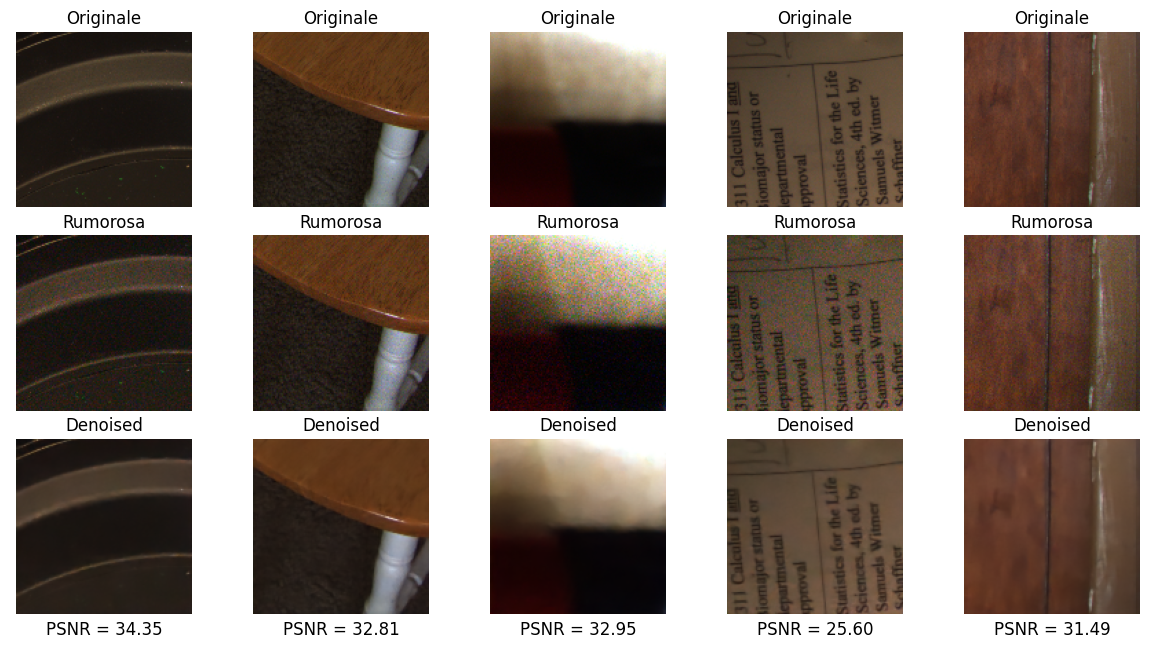
\includegraphics[width=\linewidth]{img/psnr/ridnet_student/renoir_student.png}
    \caption{Dataset Renoir}
  \end{subfigure}

  \par\vspace{4ex}

  \begin{subfigure}{0.5\textwidth}
    \centering
    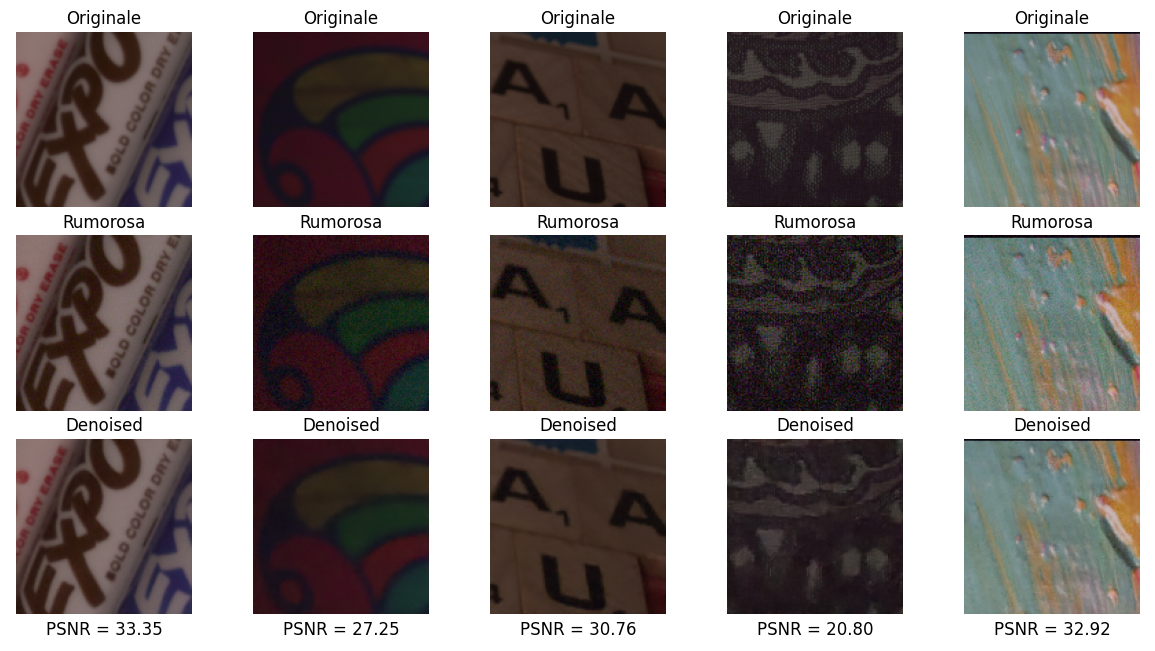
\includegraphics[width=\linewidth]{img/psnr/ridnet_student/sidd_student.png}
    \caption{Dataset SIDD}
  \end{subfigure}
  \caption{Risultati della Ridnet con iperparametri ottimizzati}
\end{sidewaysfigure}


% -------------------------------------------------------
% Dataset con tre livelli di rumore
\begin{sidewaysfigure}[h!]
    \centering
    \foreach \n [count=\i] in {15,25,50}{%x
        \begin{subfigure}{0.48\textwidth}
            \centering
            \includegraphics[width=\linewidth]{img/psnr/ridnet_student/bsd_\n_student.png}
            \caption{$\sigma=\n$}
        \end{subfigure}\hspace{2em}%
        % Vai a capo dopo ogni 2 immagini
        \ifnum\i=2 \par\vspace{2ex}\fi
    }
    \caption{Dataset BSD500 – Confronto Ridnet Student ai diversi livelli di rumore.}
\end{sidewaysfigure}

\begin{sidewaysfigure}[h!]
    \centering
    \foreach \n [count=\i] in {15,25,50}{%x
        \begin{subfigure}{0.48\textwidth}
            \centering
            \includegraphics[width=\linewidth]{img/psnr/ridnet_student/fivek_\n_student.png}
            \caption{$\sigma=\n$}
        \end{subfigure}\hspace{2em}%
        % Vai a capo dopo ogni 2 immagini
        \ifnum\i=2 \par\vspace{2ex}\fi
    }
    \caption{Dataset MIT Adobe FiveK – Confronto Ridnet Student ai diversi livelli di rumore.}
\end{sidewaysfigure}

\begin{sidewaysfigure}[h!]
    \centering
    \foreach \n [count=\i] in {15,25,50}{%x
        \begin{subfigure}{0.48\textwidth}
            \centering
            \includegraphics[width=\linewidth]{img/psnr/ridnet_student/div2k_\n_student.png}
            \caption{$\sigma=\n$}
        \end{subfigure}\hspace{2em}%
        % Vai a capo dopo ogni 2 immagini
        \ifnum\i=2 \par\vspace{2ex}\fi
    }
    \caption{Dataset Div2K – Confronto Ridnet Student ai diversi livelli di rumore.}
\end{sidewaysfigure}
  
\clearpage

\section{Risultati Fine Tuning con iperparametri ottimizzati}
\label{chap:risultati_finetune_iperparametri}

\begin{sidewaysfigure}[h!]
    \centering
    \foreach \n [count=\i] in {15,25,50}{%x
        \begin{subfigure}{0.48\textwidth}
            \centering
            \includegraphics[width=\linewidth]{img/psnr/ridnet_student/kvasir_pre_\n_student.png}
            \caption{$\sigma=\n$}
        \end{subfigure}\hspace{2em}%
        % Vai a capo dopo ogni 2 immagini
        \ifnum\i=2 \par\vspace{2ex}\fi
    }
    \caption{Dataset Kvasir pre Fine tuning – Confronto Ridnet Student ai diversi livelli di rumore.}
\end{sidewaysfigure}

\begin{sidewaysfigure}[h!]
    \centering
    \foreach \n [count=\i] in {15,25,50}{%x
        \begin{subfigure}{0.48\textwidth}
            \centering
            \includegraphics[width=\linewidth]{img/psnr/ridnet_student/kvasir_post_\n_student.png}
            \caption{$\sigma=\n$}
        \end{subfigure}\hspace{2em}%
        % Vai a capo dopo ogni 2 immagini
        \ifnum\i=2 \par\vspace{2ex}\fi
    }
    \caption{Dataset Kvasir post Fine tuning – Confronto Ridnet Student ai diversi livelli di rumore.}
\end{sidewaysfigure}



\chapter{Ringraziamenti} 
Ringrazio la Prof. Lazzaro per la supervisione e aver sopportato la mia follia.\\
Grazie agli amici conosciuti in università: Serafino, Laura e Sofia per avermi aiutato ad andare avanti in questa pazza università aiutandomi con consigli, appunti e pazienza.\\
Un grazie speciale ai miei genitori, che mi hanno supportato e sopportato durante questo periodo folle.\\
Grazie ai quei tre amici che mi ritrovo dalle superiori che non ho capito come facciano ancora a sopportarmi: Monte, Pode e Pane.\\
Grazie alla vecchia guardia di S.P.R.I.Te, Andrea LR, FraDente, Delu, Perla, Cesca ed EleRizz per avermi aiutato in un modo o nell'altro sia con esami che solo qualche chiaccherata.\\
Anche alle nuove leve di S.P.R.I.Te per i bei momenti passati insieme.\\
Infine, un grazie a tutte le persone conosciute in questo periodo, che mi hanno fatto sorridere e divertire, e capire tante cose di me, rendendo questa esperienza indimenticabile.
\center{\Large{\textbf{Grazie a tutti voi.}}}
